% !TEX TS-program = pdflatexmk
\documentclass[12pt]{article}
\usepackage{float}

\usepackage{amsthm}

% Layout.
\usepackage[top=.75in, bottom=0.75in, left=.75in, right=.75in, headheight=1in, headsep=6pt]{geometry}

\usepackage{fancyhdr, enumerate,multirow}
% Fonts.
\usepackage{mathptmx}
\usepackage[scaled=0.86]{helvet}
\renewcommand{\emph}[1]{\textsf{\textbf{#1}}}

% Misc packages.
\usepackage{amsmath,amssymb,latexsym}
\usepackage{graphicx,tikz}
\usepackage{array}
\usepackage{xcolor}
\usepackage{multicol}
\usepackage{tabularx,colortbl}
\usepackage[T1]{fontenc}
\usepackage{enumitem}
%to make tikz pics work
\usepackage{tikz,pgfplots}

\usepackage{varwidth}
\usepackage{verbatim}
\usepackage{mathtools}
\DeclarePairedDelimiter\ceil{\lceil}{\rceil}
\DeclarePairedDelimiter\floor{\lfloor}{\rfloor}

\newenvironment{centerverbatim}{%
  \par
  \centering
  \varwidth{\linewidth}%
  \verbatim
}{%
  \endverbatim
  \endvarwidth
  \par
}

\makeatletter
\newenvironment{centeredverbatim}{\expandafter\verbatim\centering}{\endverbatim}
\makeatother


\usetikzlibrary{arrows}
\newcommand{\midarrow}{\tikz \draw[-triangle 90] (0,0) -- +(.1,0);}

\usepackage[colorlinks=true]{hyperref}

% Paragraph spacing
\parindent 0pt
\parskip 6pt plus 1pt
\def\tableindent{\hskip 0.5 in}
\def\ts{\hskip 1.5 em}

\usepackage{fancyhdr}
\pagestyle{fancy} 
\lhead{\large\sf\textbf{MATH 663 }}
\rhead{\large\sf\textbf{Fall 2023}}
\chead{\large\sf\textbf{HW 8}}

\newcommand{\localhead}[1]{\par\smallskip\textbf{#1}\nobreak\\}%
\def\heading#1{\localhead{\large\emph{#1}}}
\def\subheading#1{\localhead{\emph{#1}}}

%% Special Math Symbol shortcuts
\newcommand{\NN}{\mathbb{N}}
\newcommand{\RR}{\mathbb{R}}

\newcommand{\rad}{\text{rad}}
\newcommand{\diam}{\text{diam}}
\newcommand\solution{\localhead{Solution:}}

%\newenvironment{clist}%
%{\bgroup\parskip 0pt\begin{list}{$\bullet$}{\partopsep 4pt\topsep 0pt\itemsep -2pt}}%
%{\end{list}\egroup}%

\usetikzlibrary{calc,arrows.meta}
%\pgfplotsset{my style/.append style={axis x line=middle, axis y line=
%middle, xlabel={$x$}, ylabel={$y$}, axis equal }}{



\begin{document}
\begin{enumerate}
	\item Give an example to show that if $G$ is allowed to have multiple edges, then $\chi'(G)$ may exceed $\Delta(G) +1$.\\
	\solution
	\begin{figure}[H]
		\begin{center}
			\caption{Multigraph $G$ with $\Delta(G) + 1 = 11$ but $\chi'(G) = 15$}
			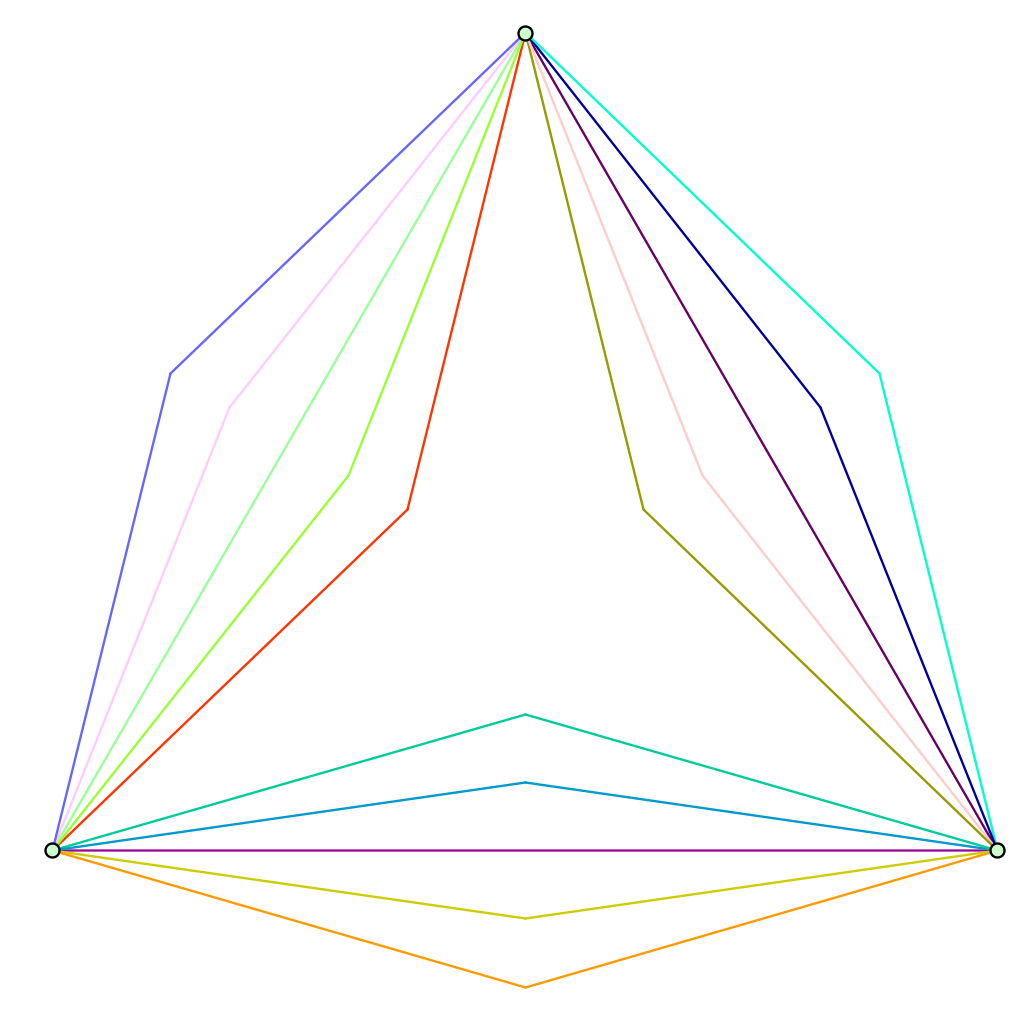
\includegraphics[width=.55\textwidth]{Multigraph.png}
		\end{center}
	\end{figure}



	\newpage
	





	\item Without using Proposition 5.3.1, show that $\chi'(G) =k$ for every $k$-regular bipartite graph $G$.
	\begin{proof} We will proceed to show that $\chi'(G) =k$ for every $k$-regular bipartite graph $G$ via induction on $k$. Consider the base case, where $G$ is a $1$-regular bipartite graph. Since every vertex is incident to exactly one edge, we can simply color all the edges the same color, an produce a 1 edge coloring, hence by Vising's Theorem $\chi'(G) =1$. 

		Suppose that $G$ is $n + 1$-regular bipartite. Since $G$ is a regular bipartite graph, it contains a one factor, $M$. Note that $G - M$ is $n$-regular bipartite since each $e \in M$ contributes one degree to exactly one vertex in $A$ and one vertex in $B$ and since $M$ spans the vertices of $G$. Now by the induction hypothesis there exists an $n$ coloring of $G - M$, call it $C$. Apply $C$ to $G$ and color the edges of $M$ the $n+1^{th}$ color, call this coloring $C'$. Note that $C'$ is a valid coloring since $M$ is a one factor. Hence by Vising's Theorem $\chi'(G) = n + 1$.
	\end{proof}
	\newpage
	







	\item Give an explicit edge-coloring to prove that the $n$-dimensional cube, $Q^n$, is Class 1.
	\begin{proof} Recall that the  $n$-dimensional cube, $Q^n$ is $n$- regular and therefore showing $Q^n$ is Class 1 is equivalent to showing $\chi'(Q^n) = n$. Now we will proceed by induction on $n$. The base case is trivial since $Q^n = K^2$, there is only one edge.... color it. Now consider $Q^{n+1}$ and recall the construction of $Q^{n + 1}$ via two copies of $Q^n$ and an independent set of edges call them $M$ (We have discussed this before and I've proven this set is independent in HW1). So $Q^{n + 1} - M$ is two components, call them $Q_1$ and $Q_2$, they are isomorphic $Q^n$ dimensional cubes and therefore $Q_1 = Q_2 = \chi'(Q^n) = n$. Apply the same edge-coloring $C$ on $Q_1$ and $Q_2$, and color the edges of $M$ the $(n + 1)^{th}$ color. Thus we have produced an edge-coloring of $Q^{n + 1}$ with $n + 1$ so by Vising's Theorem $\chi'(Q^{n+1}) = n+1$.
	\end{proof}
	\newpage
	










	\item Prove that if $G$ is a regular graph with a cut vertex, then $\chi'(G) > \Delta(G)$.
	\begin{proof} Suppose $G$ is a $k$-regular connected graph, with $\chi'(G) = \Delta(G) = k$. We will proceed to show that $G$ has no cut vertex, by proving $G$ is 2-connected. Since $G$ is $k$-regular and $k$-edge colorable for every $u, v \in G$ and for all $\alpha, \beta \in [k]$ there exists an $\alpha,\beta$ alternating $uv$-path. Now let $u, v \in G$ and consider the $\alpha,\beta$ alternating $uv$-path. Regardless of the edge color entering $v$, there exist an edge of the other color leaving $v$ and entering another vertex, not on the path. Since the $\alpha,\beta$ color classes span the graph $G$, the path can be extended to eventually enter $u$ via a $\beta$ edge, forming a cycle. Hence $G$ is 2-connected. 
 




	\end{proof}

	The rest is for my own good. \\


	Since $G$ is $k$-regular and $k$-edge colorable we know that for every $\alpha \in [k]$ the set of all $\alpha$-edges is a one-factor by regularity, and even further for every pair of $\alpha, \beta \in [k]$ the set of all $\alpha$-edges is disjoint from the set of all $\beta$-edges by being $k$-edge colorable. Thus we can conclude that the subgraph formed by all $\alpha$-edges and $\beta$-edges is connected and spans the vertices of $G$ and clearly any path between two vertices will be alternating $\alpha, \beta$.
	
	\newpage



	\item The \emph{cartesian product} of two graph $G$ and $H$, denoted $G \: \square \: H,$
	is the graph with vertex set $V(G \: \square \: H)=V(G) \times V(H).$ A pair of vertices $(x_1,y_1), (x_2,y_2)$ are adjacent in  $G \: \square \: H$ if and only if $x_1=x_2$ and $y_1y_2 \in E(H)$ or $x_1x_2 \in E(G)$ and $y_1=y_2.$
	\begin{enumerate}
	\item Draw $P_2 \: \square \: C^4.$
	\solution 
	\begin{figure}[H]
		\begin{center}
			\caption{$P_2 \: \square \: C^4.$}
			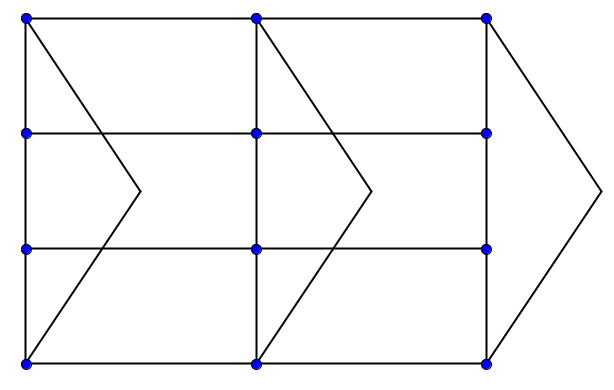
\includegraphics[width=.45\textwidth]{CartProd.png}
		\end{center}
	\end{figure}



	\item Prove that $\Delta(G \: \square \: H)= \Delta(G) + \Delta(H)$
	\begin{proof}
		
		Let $G$ and $H$ be simple graphs, and let $(u,v) \in V(G \: \square \: H)$. By definition, each adjacency of $u$ in $G$, and $v$ in $H$, induces an adjacency of $(u, v)$ in $G \: \square \: H$, so it follows that $d((u, v)) = d(u) + d(v)$. Clearly it follows that, $\Delta(G \: \square \: H)= \Delta(G) + \Delta(H)$. 
	\end{proof}
		





	\item Prove that if $\chi'(H)=\Delta(H)$, then $\chi'(G \: \square \: H)=\Delta(G \: \square \: H).$
	\begin{proof} Suppose $\chi'(H)=\Delta(H)$. Now consider $(u, v) \in G \: \square \: H$ such that $u \in G$ and $v \in H$ have maximum degree. Color every copy of $G$ in $G \: \square \: H$ with $\Delta(G) + 1$ colors. Now note that for every $u \in V(G)$ there exists at least one unused color across all copies of $u$ in  $G \: \square \: H$, call this color $c_u$. For every $u \in V(G)$ color the graph $H$ incident to every copy of $u$ with $\Delta(H)-1$ new colors and the corresponding unused color $c_u$. Thus we have constructed a $\delta(G) + 1 + \delta(H) - 1 = \Delta(G) + \Delta(H) =\Delta(G \: \square \: H)$ coloring of $G \: \square \: H$.
		
	\end{proof}
	\end{enumerate}
	\newpage










	\item
	\begin{enumerate}
	\item Let $G_1$ be a 5-cycle with one chord. Show that there exists a graph $H$ such that $L(H)=G_1.$
	\solution
	\begin{figure}[H]
		\begin{center}
			\caption{Graph $G_1$ in Red and $H$ in Blue.}
			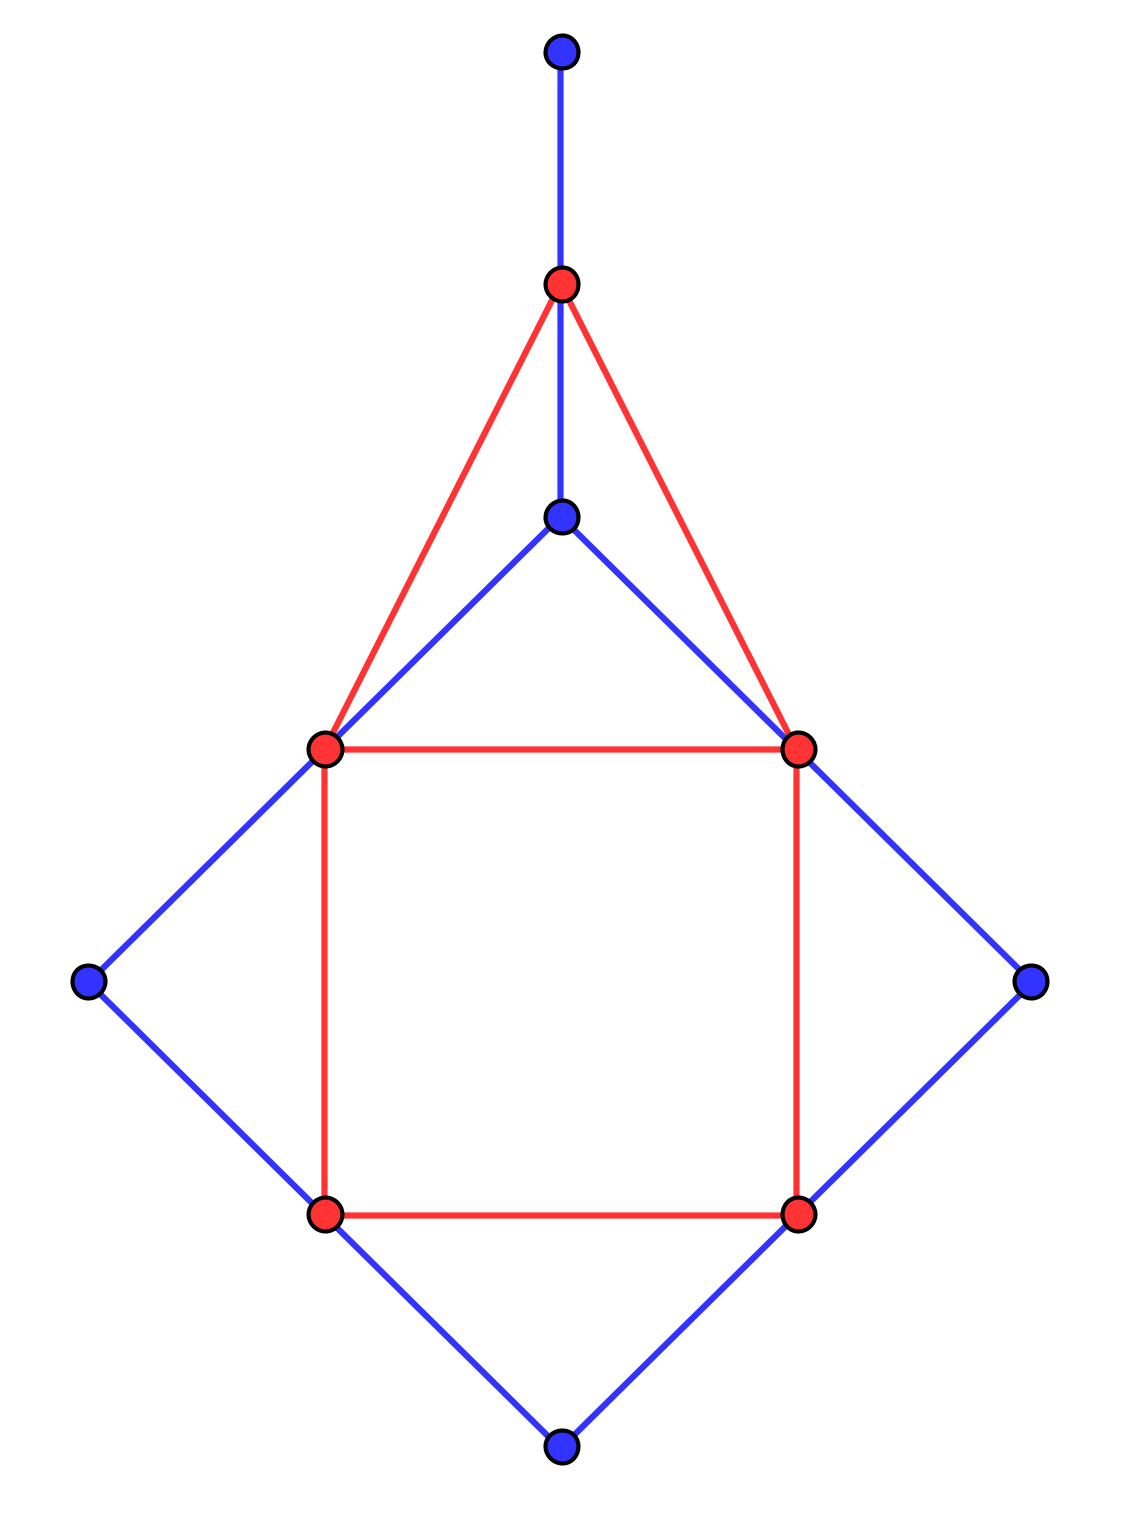
\includegraphics[width=.35\textwidth]{CycleGraph.png}
		\end{center}
	\end{figure}


	\item Prove that for the graph $G_2$ (drawn below) that there does not exist any graph $H$ such that $L(H)=G_2.$\\
	\begin{figure}[H]
		\begin{center}
			\caption{Graph $G_2$}
			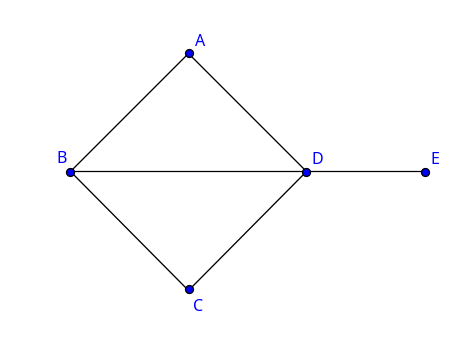
\includegraphics[width=.35\textwidth]{ClawGraph.png}
		\end{center}
	\end{figure}


	\begin{proof} 
		Suppose for the sake of contradiction that there exists a graph $H$ such that $L(H) = G_2$. Clearly the part of $G_2$ which is a 4-cycle with a chord can be a line graph via a similar construction as the previous problem. However to incorporate vertex $E$ into the line graph, would also add an edge $CE$ or $AE$. 
		\begin{figure}[H]
			\begin{center}
				\caption{Graph $G_2$ in Red and $H$ in Blue}
				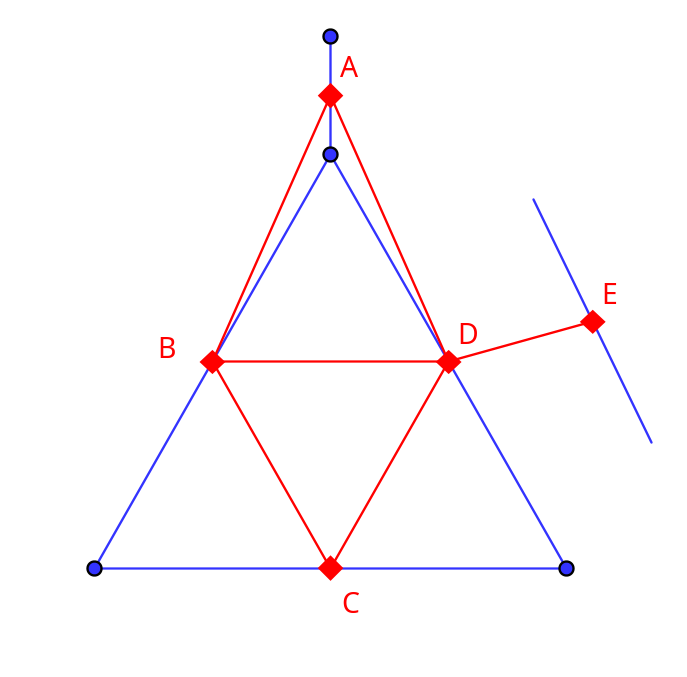
\includegraphics[width=.40\textwidth]{ClawLineGraph.png}
			\end{center}
		\end{figure}



	\end{proof}
	
	
	\end{enumerate}
\end{enumerate}
\end{document}